\documentclass[a4paper,10pt]{article}
\usepackage{hcolor}
\usepackage{color}
\usepackage{fancyhdr}
\usepackage[pdftex]{graphicx}
\usepackage[]{graphicx}
\def\RCS$#1: #2 ${\expandafter\def\csname RCS#1\endcsname{#2}}
\RCS$Date$
\RCS$Revision$


% for pdflatex only
\newif\ifpdf
\ifx\pdfoutput\undefined
\pdffalse % we are not running PDFLaTeX
\else
\pdfoutput=1 % we are running PDFLaTeX
\pdftrue
\fi
\ifpdf
\pdfinfo{ /Author (Thomas Cokelaer)
          /Title (BankEfficiency documentation)
}
\usepackage[pdftex,plainpages=false,pdfpagelabels,hypertexnames=false,
colorlinks=true,pdfstartview=FitV,linkcolor=blue,citecolor=blue,urlcolor=blue]{hyperref}
\usepackage{thumbpdf}
\else
\usepackage{hyperref}
\fi





\setlength\topmargin{0in}
\setlength\headheight{0in}
\setlength\headsep{0.2in}
\setlength\textheight{24cm}
\setlength\textwidth{6.5in}
\setlength\oddsidemargin{0in}
\setlength\evensidemargin{0in}
\setlength\parindent{0.25in}
\setlength\parskip{0.25in}


\newcommand{\code}[1]{%
\begin{center}
  \fboxsep=10pt
  \fcolorbox{black}{yellow}
  { \parbox[c]{12cm}{ \color{blue}{#1}}}
\end{center}}

\newcommand{\insp}{\textsc{inspiral}~}
\newcommand{\bank}{\textsc{bank}~}
\newcommand{\noise}{\textsc{noisemodels}~}
\newcommand{\be}{\textsc{BankEfficiency}~}

% Title Page
\title{BankEfficiency documentation}
\author{Thomas Cokelaer}

\begin{document}
\bibliographystyle{unsrt}
\pagestyle{plain}
\fancypagestyle{plain}
\rfoot{}
\cfoot{\arabic{page} of \pageref{theend}}
\lfoot{}
\pagestyle{plain}
\lhead{BankEfficiency documentation -- v.\RCSRevision}


\noindent
\maketitle

%\addcontentsline{toc}{section}{References}
\setcounter{tocdepth}{1}
\tableofcontents
%\addcontentsline{toc}{section}{References}
\section{Introduction}
\be is a tool written in C that is available in \textsc{lalapps/src/findchirp/}. It was primary developped to test efficiencies of the template bank placement coded in LAL, in the context of detection of inspiralling compact binaries in ground based detetectors. 

Although \be heavily relies on LAL packages such as the \bank, \insp and \noise packages, nevertheless it has its own sets of routines, which makes \be a pretty long piece of code (about 4,000 lines) but also a quite independant one.  Despite this relative length, I tried to make \be as modular as possible; the main core is only about 400 lines. It should therefore be easy to adapt it to your needs if you know the packages mentionned here above. 

\subsection*{What BankEfficiency can do :}
\begin{itemize}
 \item Compute overlaps between a signal and a template bank.
 \item Perform large Monte-Carlo simulations using \textsc{CONDOR} and \textsc{DAG} technologies.
 \item Store results in XML format both for data mining and keeping track of the parameters being used.
 \item Inject any type of signal that is available in LAL \insp package.
 \item Use any template bank that is available in LAL \bank package.
 \item Use any noise model that is available in LAL \noise package.
\end{itemize}

\subsection*{What BankEfficiency cannot do }
\begin{itemize}
 \item Multidetector analysis.
 \item Analyse real noise, although implementation of an interface should be straigtforward.
 \item PTF filtering.
 \item BCV spin filtering.
\end{itemize}

\subsection*{What BankEfficiency has done}
\begin{itemize}
 \item Validation of the SPA template bank coded in LAL \bank package, based on a square lattice for the SPA templates \cite{squarebank}, which has been used in LIGO and GEO600 science runs up to S4.
 \item Design and validation of the SPA template, based on hexagonal lattice for the SPA templates. It has also show the possibility to use other models such as EOB, PadeT1 with the same template bank \cite{hexabank}, which is currently used in S5 analysis.
\item Design and validation of the BCV template bank used in S2/S3/S4 LIGO BBH searches \cite{bcvbank}
\item Overlaps of eccentric models with SPA template bank.
\end{itemize}


\be has become a powerful tool. However, its complexity implies a lot of input arguments, most of them having default values hardcoded. This documentation is aimed at
\begin{enumerate}
 \item Explaining what type of simulations you can performed by showing concrete examples.
 \item Describing the input parameters in details.
 \item Describing the output files.
 \item Explaining how to run simulations using CONDOR/DAG.
\end{enumerate}

In the following we assume that the reader knows what is a template bank, what is matched filtering, what is a template, and what are the models such as EOB, PadeT1, TaylorT1 and so on. If not, you may look at one of the references in the bibliography.

\section{Tutorial}
In this section, I provide a few example on how to use \be. This selection will explain you how to set the parameters and what are the output files. This is of course a non exhaustive list of what can be done. 

\subsection{First example and outputs}
Let us start with a very simple example that has only two input parameters. This is possible because all parameters have default values. With the following command, we specify explicitly that both the signal and template approximant are based on EOB model:

\code{lalapps\_BankEfficiency {-}{-}template EOB {-}{-}signal EOB}

Concerning the signal there is no ambiguity:  the argument 
\textbf{{-}{-}signal EOB} means that all injected waveforms are based on EOB model. However, concerning the argument \textbf{{-}{-}template EOB}, one need to understand that it sets both the template model and the template bank placement. For instance, if the template is BCV, then the template bank is a BCV template bank as well. For all other approximant such as EOB, PadeT1, TaylorF2 (physical models) then the template bank is the standard SPA template bank. We'll come back on template bank placement in the next sections.

Note that the component masses of the injected signal are randomised so that the total mass is uniformly distributed. By default, component masses are between 5 and 20 solar masses. The phase order of both the signal and templates are set to 2PN order by default. There are many other default values such as the sampling, the minimal match of the template bank\dots We'll see in Sec.\ref{default} how to change all these default values.

\textbf{Note that by default the initial phase of the signal is randomised but can be switch off (and set to zero) using \textbf{{-}{-}no-start-phase} option}

The previous command returns a bunch of numbers on the screen. If not, most probably there was an error in the code.You may use the option \textbf{{-}{-}debug 33} to check any standard LAL errors. I would advice to always use this option.

The next step is to understand what all these numbers are. From the output on the screen this is quite tedious. Luckily, at the end of the previous command, one can add an option to stored results in an XML file : \textbf{--xml-output} such as in the following example

 \code{lalapps\_BankEfficiency {-}{-}template EOB {-}{-}signal EOB {-}{-}debug 33 {-}{-}xml-output}

This option will create a file called \textbf{BankEfficiency-Result.xml} that contains (1) all the input parameters (including the default values) and (2) all the results of the simulation. The structure of the XML file is similar to all standard LIGO XML file. Therefore, one can use tools such as \textsc{lwtprint} from ligotools. The output results of \be are stored in XML format in a table that is called \textbf{bankefficiency} (no big caps). From now, you can extract the output of \be using this kind of command: 

\code{lwtprint BankEfficiency-Result.xml -t bankefficiency -c mass1\_sim, mass2\_sim, snr}

where \textbf{-t bankefficiency } parses the \be outputs and \textbf{-c snr,mass1\_sim,mass2\_sim} means you want to extract the columns labelled \textbf{snr}, \textbf{mass1\_sim} and \textbf{mass2\_sim}. Of course, you need to know what are the column's name. At the end of this document (Sec.~\ref{default}), we provide the list of columns and their meanings. You can also edit the XML file and figure out by yourself.  

In the previous example, we extracted the component masses as well as the field called \textbf{snr}. By SNR, we actually mean the max SNR over the entire template bank. This is a single number for each injected signal. This number is the maximisation over time and parameter space of all the correlations. 

As you've probably noticed, the input parameters can be very succint. In the first example, we provided only 2 or 3 arguments. This simply means that many parameters are set by default. For instance the sampling is 2048Hz and  the template bank is based on a square placement and so on. In order to know all the default values, you can consult the header of \be. A nicer way is again to look at the XML file. Indeed, all the parameters used for the simulation are stored in the \textbf{process\_params} table together with the version of the code that has been used, which is stored in the \textbf{process} table. So, using the process\_params table you should be able to reproduce your results. 

If you use \textbf{BankEfficiency} as a standalone code and add the option \textbf{--print-bank}, you will also have the template bank stored in a file called \textbf{BankEfficiency-Bank.xml} as welll as in ASCII format (\textbf{BankEfficiency-Bank.dat}).

There are a few other possible outputs and we will come back to this later in this document.


\subsection{How to test a template bank}
\be was designed to test the efficiency of a template bank. To do so, you need to inject many signals, and filter them one by one through all the template bank. 

There are three important steps : 
\begin{enumerate}
 \item Set the signal model and its parameters
 \item Set the template and its parameters
 \item Set the template bank and its parameters
\end{enumerate}

The two last points seem similar (dealing with the template) but are completely independant. The template bank is a grid of points in the parameter space considered (e.g., component masses) and the template model can be anything. Ideally, the template bank should be constructed with the knowledge of template model. This is the case for the so-called SPA tempalte bank that is designed for TaylorF2 model. However, since other model such as TaylorT3, EOB are quite similar to the TaylorF2, you can use the same so-called SPA template bank for those models as well. 

Nothing prevent you to use this SPA template bank (the grid) with model based on something that can be very different such as Eccentric or amplitude corrected waveforms.

So, coming back to the template bank test, one really need to inject many signals to be able to quantify the efficiency of the template bank, that is the distribution of the overlaps in the parameter space. To do so, you can set the number of simulations using  \textbf{--n 10000}. 

Then, to be realistic, the minimal match of the bank is set to \textbf{-- mm 95\%} (by default it is set to 80\%).

\code{lalapps\_BankEfficiency {-}{-}template EOB {-}{-}signal EOB  {-}{-}xml-output {-}{-}print-bank {-}{-}debug 33 {-}{-}n 10000 {-}{-}mm 0.95}

This command returns 10000 lines of numbers. So again, it is better to work with the XML file. \be does not create any plots for you. So you can use whatever tool you prefer (MATLAB, XMGrace,\dots). However, within \textsc{lalapps/src/findchirp} package, there are 2 python files called plotbankefficiency.py (the executable) and inspiraltools.py (the library). Use the former one as follows : 

\code{python plotbankefficiency.py --glob 'BankEfficiency-Results.xml' --verbose --user-tag 'test'} so as to generate a bunch of plots you may found useful. For instance, Fig.\ref{fig:snr1} shows the distribution of the overlaps versus total mass.

\textbf{inspiraltools.py requires a few python packages that you may not have by default (scipy, delaunay, ...), in particular for the contour and scatter plots. Please update your packages. }

\begin{figure}
\centering
 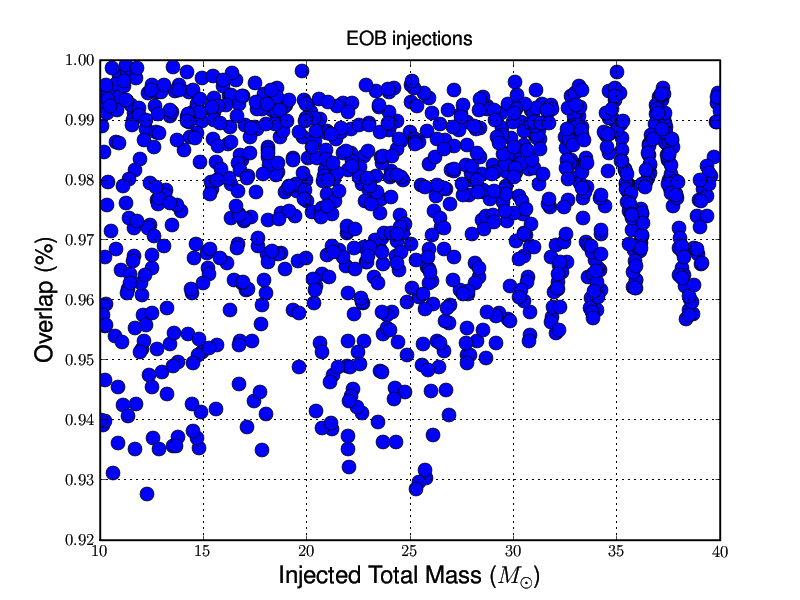
\includegraphics[width=0.4\textwidth]{bankefficiencydoc_snr_versus_totalmass}
\caption{\label{fig:snr1} Overlaps versus total mass of the injected signals.}
\end{figure} 

Note that the XML table does not contains all the physical information you may want. It is quite light though because only 2 mass parameters are stored for the injection and for the template that gives the best SNR. Indeed, other set of parameters can be computed a posteriori.

\subsection{Noise and Signal}\label{model}
In the two previous examples, we considered noiseless simulations. \be was indeed created to check the overlaps between a template bank and injections. So there was no need for noise. However, the \textsc{noisemodel} package has also the possibility to inject a signal into noise (you can even set the signal amplitude to be null so as to study only the noise).  This can be done as follows : 
\code{lalapps\_BankEfficiency {-}{-}template EOB {-}{-}signal EOB {-}{-}debug 33  {-}{-}mm 0.95 {-}{-}n 10000  {-}{-}xml-output {-}{-}print-bank  {-}{-}simulation-type NoiseAndSignal {-}{-}signal-amplitude 25}

The \textbf{{-}{-}simulation-type} can be set to [NoiseOnly,NoiseAndSignal,SignalOnly(default)]. The last option \textbf{{-}{-}signal-amplitude} set the average SNR of the signal. The default spectrum used inside the matched filtering or to define the noise spectrum is the initial LIGO by default.

The NoiseAndSignal case is very useful to perform test of the Fisher matrix by testing the dispersion/accuracy of the mass parameters. However, in such a case, you would want the mass of the injection to be fixed instead  of being randomized. This can be done by fixing the individual masses as follows: 

\code{lalapps\_BankEfficiency {-}{-}template EOB {-}{-}signal EOB {-}{-}mm 0.95 {-}{-}n 10000  {-}{-}xml-output {-}{-}print-bank  {-}{-}simulation-type NoiseAndSignal {-}{-}signal-amplitude 25 {-}{-}m1 10 {-}{-}m2 10}

Another option related to the noise is that you may want to specify different type of colored noise, which currently are LIGOI, LIGOA, VIRGO, EGO, TAMA for initial LIGO, advanced LIGO, VIRGO, Einstein Telescope and TAMA, which can be set using \textbf{{-}{-}noise-model}.


\code{lalapps\_BankEfficiency {-}{-}template EOB {-}{-}signal EOB {-}{-}mm 0.95 {-}{-}n 10000  {-}{-}xml-output {-}{-}print-bank  {-}{-}simulation-type NoiseAndSignal {-}{-}signal-amplitude 25 {-}{-}m1 10 {-}{-}m2 10 {-}{-}noise-model LIGOA}

Using the \textbf{{-}{-}print-psd} option, the PSD will be saved in \textbf{BankEfficiency-PSD.dat}.

\subsection{Template bank related}\label{bank}
Let us now look in more details at the parameters related to the template bank itself.

First of all, there are only two specific type of template bank available at the moment that are in the LAL \bank package. The first template bank is the SPA template bank for physical models such as EOB, Taylor, Pade model. The second one is a BCV template bank that is created if \textbf{{-}{-}template} is set to \textbf{BCV}. Let us focus on the SPA template bank for now. 

There are two types of placements : square and hexagonal. Historically, square placement was implemented first and can be called using \textbf{{-}{-}bank-grid-spacing SquareNotOriented}. Then hexagonal placement was imlemented and can be called using \textbf{{-}{-}bank-grid-spacing Hexagonal}

\textbf{Technical:}
A template bank is constructed using the metric components of the signal/template manifold. The metric components are computed by calculating quantities such as the moments, which in turn are integrals from a lower cut-off frequency to an upper cutoff frequency. The latter is  by default set to the  Nyquist frequency (so be aware that the sampling is 2048Hz by default). One can force the upper cut-off frequency to be a fixed value by setting \textbf{{-}{-}bank-ffinal}. One can also recompute the moments for each template so that the upper cutoff frequency used to compute the moments is the last stable orbit instead of the Nyquist frequency. This option is not yet fully implemented within the template bank code but can be set on for the Gammas only (does not change the placement but affect the gammas and therefore the ematch values) using \textbf{{-}{-}compute-moments}.

By default the minimal match of the template bank is 80\% but you can change it using \textbf{{-}{-}mm} option.

To set the masse range to which the bank is efficient, use \textbf{{-}{-}bank-mass-range a b}, where \textbf{a} and \textbf{b} are 2 sorted values of component mass.

There is also the possibility to create a template bank, which is a simple box in $\tau_0/\tau_3$ that has a fine grid. The fine grid is implemented within \be and requires these parameters: 
\begin{itemize}
 \item \textbf{{-}{-}t0-fine-range} Two values to set the t0 range.
\item \textbf{{-}{-}t3-fine-range} Two values to set the tau3 range.
\item \textbf{{-}{-}t0-fine-bin} Number of bins in this dimension.
\item \textbf{{-}{-}t3-fine-bin} Number of bins in this dimension.
\end{itemize}



\subsection{Eccentricity related}\label{eccentricity}
If the signal is set to \textbf{Eccentricity} (using the {-}{-}signal option), then you can set the initial eccentricity of the simulated signals by using a range. The eccentricity will be uniformly distributed witin the two values that define this range. For instance :
\code{lalapps\_BankEfficiency {-}{-}template TaylorT3 {-}{-}signal Eccentricity {-}{-}mm 0.95 {-}{-}n 10000  {-}{-}xml-output --signal-eccentricity-range 0 0.4}

Note that the Eccentric model is only implemented at the Newtonian order for the moment. Therefore, one must specify the Newtonian order on the command line argument (by default the 2PN is used). If not, the code will fail. 

So, stricly speaking, the command above should have been : 
\code{lalapps\_BankEfficiency {-}{-}template TaylorT3 {-}{-}signal Eccentricity {-}{-}mm 0.95 {-}{-}n 10000  {-}{-}xml-output --signal-eccentricity-range 0 0.4 --signal-order 0}

where the number 0 stands for Newtonian.

There is no proper eccentric template bank. However, one can set the template bank to be based on SPA bank (optimised for a search that uses 2PN templates) but place an eccentric template on each point of the grid. Yet, by default all templates will have their eccentricity fixed to zero. So, really, this is not an eccentric template bank. One would need the metric in the eccentric dimension and create a template bank adequately. Yet, there is a naive template bank that is called by using the option \textbf{{-}{-}bank-eccentricity-range} followed by a range of values and a number of bins. The template will be \textbf{bins} times the original template bank each of them having a different value of eccentricity. This is naive because it assumes that the metric is flat in the eccentric dimension even though this is clearly not the case. However, one can already test how we can recover eccentric waveforms with eccentric templates and performed some tests. To set the number of layers/bins, use \textbf{{-}{-}bank-eccentricity-bins}.

\code{lalapps\_BankEfficiency {-}{-}template TaylorT3 {-}{-}signal Eccentricity {-}{-}mm 0.95 {-}{-}n 10000  {-}{-}xml-output --signal-eccentricity-range 0 0.4 --signal-order 0 --bank-eccentric-range 0 0.4 --bank-eccentricity-bins 10}

\subsection{BCV related functions}\label{bcv}
In this section, we show how to test a template bank based on BCV template and how a BCV template bank can detect signals based on other models such as EOB, PadeT1, \dots. 

I will not described the placement itself neither the filtering (see for instance Ref.~\cite{bcvbank}). Here is just a simple example: 

\code{./lalapps\_BankEfficiency --template BCV --bank-alpha 0.01 --bank-psi0-range 10 250000 --bank-psi3-range -2000 -10 --bank-fcut-range 2 6 --bank-number-fcut 3 --bank-inside-polygon 1 --signal EOB --signal-mass-range 5 20 --xml-output}

The BCV signal can be injected as well. We can force the psi0/psi values using \textbf{{-}{-}psi0} and \textbf{{-}{-}psi3} options. 
Otherwise the \textbf{{-}{-}signal-psi0-range} and \textbf{{-}{-}signal-psi3-range} need to be fixed or default values will be used instead.

Concerning the filtering there is an option to avoid the alpha constraint to be used \textbf{{-}{-}no-alpha-constraint} \textbf{{-}{-}alpha-constraint}.

The template bank can be either Hexagonal or Square, but only the Hexagonal case has been tested exhaustively. 

The filtering may fail if the psi0/psi3 pair gives an ending frequency lower than the lower cut-off frequency. 

\subsection{Amplitude Corrected related}\label{ampcor}
To use the amplitude corrected waveforms, one can simply set the signal to be \textbf{AmpCorPPN}. The order needs also to be set by using \textbf{{-}{-}signal-amp-order}  and \textbf{{-}{-}template-amp-order}

Concerning the input parameter of the signal, one also need to set the range of inclination and polarisation using \textbf{{-}{-}signal-inclination-range} and \textbf{{-}{-}signal-polarisation-range}. 

\textbf{Check this : Note, however, that because the signal is normalised with respect to their energy, the effect of the inclination on the amplitude of the signal won't be seen !}

The template bank is based on SPA placement.

The filtering is the standard filtering in quadrature. 

\subsection{Others issues}\label{others}
There are a few other options. Some of which can be useful.
\subsubsection{Change the length of the vectors}
In principle \be estimates the longest length of all templates and all possible signals and allocate memory such that the vectors are long enough. If you still want to increase the size of the vectors  you can use \textbf{{-}{-}num-seconds} to fix the size yourself (but you need to know the optimal length).

\subsubsection{Lower cut off frequencies}
To set the lower cut-off frequency, use \textbf{{-}{-}fl}, which affects both the signal and template lower cut-off frequency. You can independantly set the template/bank cut-off frequency and signal lower cut off frequency using \textbf{{-}{-}template} and \textbf{{-}{-}signal}.

\subsubsection{Fast option}
There is a fast option to perform the simulation quicker that can be very powerful. It is based on the metric of the signal. So if the template and the signal are based on the same approximant, it can be used very safely. It is switched on by using \textbf{{-}{-}fast-simulation EMatch} and \textbf{{-}{-}e-match}, which is set to 0.5 by default

\code{./lalapps\_BankEfficiency --fast-simulation EMatch --e-match 0.5 --xml-output}


The match is unity when the signal and template are identical. As soon as they differ, the match decreases. Since it is not normalised, it can take negative values. Also, in the xml table, we store the number of templates that have been used in the \textbf{nfast} field.

How does the EMatch option works ? First, we know the position of the signal $s$. So, we compute the Ematch between this signal and a template. If the ematch value is greater than the ematch parameter (e.g. 0.5), then we compute the overlap between the signal and the template otherwise we skip the filtering. 

Another fast option is the Heuristic1 one. This is very similar to the EMatch case but the ematch value is computed between the template and the position of the template that gave the best SNR up to now. The ematch argument is not used. The consequence is that we can go much farther that the original position of the signal. This is useful in the presence of noise or when signal and template differ significantly. Typically, I use this option when signal is Eccentricity and template is non Eccentric waveforms. If you use this option, you also need to stop the simulation at some point. This is done by setting the \textbf{--fast-param1} option (default of 50). THis argument means that if after 50 iterations, no filtering gave a larger SNR that the current maximum SNR then we stop the template bank parsing.



 

\subsubsection{BHNS injections}
There are many ways to choose the parameters of the signal to be injected. By default, the total mass is uniformly distributed and the component masses are set using the option \textbf{{-}{-}signal-mass-range}. You can overwrite this option by using together the \textbf{{-}{-}m1} and \textbf{{-}{-}m2} options to force the component masses to be fixed. Similarly, if you prefer to work with the chirp times parameters, you can use 
\textbf{{-}{-}tau3} and \textbf{{-}{-}tau0}. Finally, there is an option to force the masses to be such that the binary system is a BHNS system, that is the first component mass in in the range $[1,3]M_\odot$ and the second component mass is larger than $3M_\odot$. This option is \textbf{{-}{-}bhns-injection}. Of course you need to be sure that \textbf{{-}{-}signal-mass-range} has a range that include the value 3.

\subsubsection{Check the code}
There is a special option that is \textbf{{-}{-}check} or equivalently \textbf{{}-{-}faithfulness}. This is a very powerful option that set the template parameter to be identical to the signal. So, you can compute the faithfulness and check your code. Ideally, the output SNRs must be equal to 1. If not something is wrong in your code, or different between the template and signal parameters. 

However, using this command :
\code{./lalapps\_BankEfficiency --template EOB --signal EOB --xml-output --n 100 --check} 
we obtain 100 SNRs that are not stricly equal to 1. The reason is that we randomize the starting phase of the signal. To remove this option, use the command \textbf{{-}{-}start-phase}. Now you should get 1 all the time. There are some other parameters that are not overwritten : lower cut-off frequency, order of the phase and the approximant.


\section{Deploy your DAGs and CONDOR jobs}\label{dagandini}
\be can be used standalone or in parallel on a cluster using \textsc{CONDOR}. Changing the seed will provide different outputs, which can be recombined all together and analysed. to do so, we will use Condor and Dagman concepts that I assume you already know.

In the \textsc{lalapps/src/findchirp} package, there is python script called \textbf{bep.py}, which can be call to automatically create a dag file. This script requires one ini file, an example of which is \textbf{bep.ini} available in the same directory. This ini file can be changed to your need. The idea is that it contains all the arguments that should be passed to \be command line argument. 


\subsection{The ini file}\label{ini}
Here is a very simple example of bep.ini file that can be used to create the dag file. 

\begin{verbatim}
[main]
executable=./lalapps_BankEfficiency

[general]
mm=0.95
sampling=2048
fl=40

[bank]
bank-grid-spacing=Hexagonal

[signal]
signal=EOB

[simulation]
ntrial=1000
njobs=100
\end{verbatim}

change it to your need. The structure of the ini file  requires to have 5 sections as shown above ([main], [bank], ...). The content of the main section must contain the argument \textbf{executables}. Other than that there is no rules with respect to the order of the arguments as far as it is a valid  argument. 

\subsection{Generate the dag files.}\label{dag}
\code{python bep.py --config-file bep.ini}

\subsection{Submit the dag}
This command 
\code{condor\_submit\_dag -maxjobs 100  -f bep.dag}
will start the \textsc{DAG}. You can see the status as usual using \textbf{condor\_q}. Once done, the \textsc{DAG} will merge all the files (bankefficiency*out) together using the script \textbf{finalise.sh}. Nothing prevent you to use it while simulations are still running. This is very convenient for those of you who wants to study the efficiencies even though all the simulations are not over. 


\section{Meaning of the bankefficiency XML table}\label{xml}
\subsection{Meaning of the bankefficiency table}
Here is the list of the current field contained within the bankefficiency XML table:
\begin{description}
\item[psi0] The first BCV parameter of the template
\item[psi3] The second BCV parameter of the template
\item[psi0\_sim] The first BCV parameter of the injection
\item[psi3\_sim] The second BCV parameter of the injection
\item[tau0] The first mass parameter of the template
\item[tau3] The second mass parameter of the template
\item[tau0\_sim] The first mass parameter of the injection
\item[tau3\_sim] The second mass parameter of the injection
\item[ecc] eccentricity of the best templates
\item[ecc\_sim] eccentricity of the signal at 2FL\_3 
\item[ecc\_sim\_fl] eccentricity of the signal at F\_L
\item[ffinal] final frequency  of the best template
\item[ffinal\_sim] final frequency of the injection
\item[mass1\_sim] The first mass parameter of the injection
\item[mass2\_sim] The second mass parameter of the injection
\item[phase\_sim] The initial phase of the injection
\item[snr] the best overlap maximised over all template bank and time
\item[snr\_at\_ta] irrelevant for now
\item[phase] the phase of the best template
\item[alpha\_f] the alpha\_f value of the best template (BCV related)
\item[time] the time of arrival of the best template
\item[time\_sim] the starting time of the signal (does not work for some models such as BCV)
\item[nfast] number of templates really used
\item[nfast] number of templates after which the max SNR was found. 
\end{description}

\subsection{How to add your own field}
Here is the brief procedure to add a new field in the table:
\begin{enumerate}
 \item Change the macros in BankEfficiency.h
 \item Change the functions PrintResults (stdout)
 \item Change the function  PrintXMLResults (XML)
\end{enumerate}


\section{Arguments and their default values}\label{default}
In the following, - or ? means this option is not fully checked.
\subsection{Bank and template related}
\begin{center}
\begin{tabular}{|l|p{6cm}|p{3cm}|c|}
\hline
argument &  description & number of argument required &default value \\ \hline
--bank-alpha & The alpha value to be used in the BCV bank & 1 &0.01 \\ \hline
--bank-fcut-range & Range of final frequnency in units of GM (e.g., 3 6)& 2& 3 6  \\ \hline
--bank-ffinal & The final frequency to be used in the moments computation (if set it is the same for all templates) &1 &Nyquist\\\hline
--bank-inside-polygon & BCV related. reject all template outside a polygon defined within \bank package & 1 boolean & 1\\\hline
--bank-grid-spacing & The template bank placement. [Hexagonal, SquareNotOriented, Square] & 1 & Square\\\hline
--bank-number-fcut & BCV related. number of layer in fcut dimension& 1&5\\\hline
--bank-mass-range &Individual mass range of the simulated events&2&5 20\\\hline
--bank-max-total-mass& to be checked&-& None\\\hline
--bank-min-total-mass&to be checked&-& None\\\hline
--bank-psi0-range &BCV related&2&10 250000\\\hline
--bank-psi3-range &BCV related&2&-2200 -10\\\hline
--bank-eccentricity-range & Range of eccentricity of the templates & 2 & 0 0.4 \\\hline
--bank-eccentricity-bins&Number of layers in the eccentric template bank&1&1\\\hline 
--mm &The minimal match of the bank&1&0.80\\\hline
--template-fl  &lower cut-off frequency of the templat &1&40\\\hline
--template  &the template approximant (EOB, Pade,...)&1&\\\hline
--template-order &the phase order of the template&1&4\\\hline
--template-amp-order &the amplitude correction of the tempalte&1&5\\\hline
--t0-fine-range &Range of tau0 values for the fine template bank&2&\\\hline
--t3-fine-range &Range of tau3 values for the fine temnplate bank&2&\\\hline
--t0-fine-bin &The number of template along tau0 &1&None\\\hline
--t3-fine-bin &The number of template along tau3. &1&None\\\hline

\end{tabular} 
\end{center}



\subsection{Signal related}
\begin{center}
\begin{tabular}{|l|p{8cm}|p{3cm}|c|}
\hline
--signal &&&EOB\\\hline
--signal-alpha& BCV related. The alphaF value of the signal&1&0.01\\\hline
--signal-amp-order&The amplitude correction order&1&5\\\hline
--signal-alpha1&obsolet&-&-\\\hline
--signal-alpha2&obsolet&-&-\\\hline
--signal-amplitude&The SNR of the signal&1&10\\\hline
--signal-eccentricity-range&The range of eccentricity of the eccentric signal. Uniformly distributed&2&0 0.4\\\hline
--signal-ffinal&Force the ffinal of the signal& 1&None\\\hline
--signal-fl 40&lower cut off frequency of the signal&1&40\\\hline
--signal-inclination-range&Inclination range of the signal&2&0 $\pi$\\\hline
--signal-polarisation-range&Polarisation range of the signal&2&0 $\pi$\\\hline
--signal-mass-range&Range og the component mass&2&5 20\\\hline
--signal-tau0-range&-&-&-\\\hline
--signal-tau3-range&-&-&-\\\hline
--signal-order&The phase order 4 means 2PN, 5 means 2.5PN and so on&1&4\\\hline
--signal-nstartpad&-&-&-\\\hline
--signal-psi0-range&BCV related.&2&10 250000\\\hline
--signal-psi3-range&BCV related.&2&-2200 -10\\\hline
--signal-random-nstartpad&?&1&None\\\hline
--signal-max-total-mass&Max total mass &1&None\\\hline
--signal-min-total-mass&Min total mass&1&None\\\hline
\hline
--tau0 &Set the injection parameters to be always equal to this value. Must be use with --tau3&1&None\\\hline
--tau3 &Set the injection parameters to be always equal to this value. Must be use with --tau0&1&None\\\hline
--psi0 &Set the injection parameters to be always equal to this value. Must be use with --psi0&1&None\\\hline
--psi3 &Set the injection parameters to be always equal to this value. Must be use with --psi0&1&None\\\hline
--m1 &Set the injection parameters to be always equal to this value. Must be use with --m2&1&None\\\hline
--m2 &Set the injection parameters to be always equal to this value. Must be use with --m1&1&None\\\hline

\end{tabular}
\end{center}

\subsection{Other options}

\begin{center}
\begin{tabular}{|l|p{8cm}|p{3cm}|c|}
\hline
--debug &Set to 33 to have LAL error, set to 6 to have memory leaking checked and so on. See LAL documentation &1&0\\\hline
--e-match  &e-match for the fast simulation option&1&0.5\\\hline
--fl &&&40\\\hline
--h &help&0&None\\\hline
--ascii2xml &Internal usage only for the DAG generation&0&None\\\hline
--ntrial,--n  &Number of simulations&1&1\\\hline
--noise-amplitude &?&?&?\\\hline
--noise-model &one of [LIGOI, LIGOA, VIRGO, GEO, EGO]&&\\\hline
--num-seconds &Set the vector duration in seconds&1&None\\\hline
--sampling &Sampling frequency&1&2048\\\hline
--seed &The seed of the random process&1&?\\\hline
--simulation-type &The type of simulations [NoiseOnly, NoiseAndSignal, SignalOnly]&1&SignalOnly\\\hline
--no-start-phase &force the initial phase to be zero all the time&0& not set\\\hline
--user-tag &not yet finalised&-&-\\\hline
--ambiguity &print the ambiguity function&0&None\\\hline
--alpha-constraint &BCV related&0&None\\\hline
--bhns-injection &inject BHNS waveforms only&0&None\\\hline
--no-alpha-constraint &BCV related&0&None\\\hline
--print-best-overlap &to check &0&None\\\hline
--faithfulness,--check &check the code&0&None\\\hline
--print-psd &print the PSD in BankEfficiency-PSD.dat&0&None\\\hline
--print-snr-histo &Save the Histogram of all the correlation in BankEfficiency-Histogram.dat&0&None\\\hline
--verbose &verbose option&0&None\\\hline
--version &print the version numbers&0&None\\\hline
--print-bank &print the tenplate bank in BankEfficiency-Bank.xml &0&None\\\hline
--compute-moments &Recompute the gamma of the template &0&None\\\hline
--xml-output &print results in an xml file BankEfficiency-Result.xml&0&None\\\hline
--print-prototype &internal usage only&0&None\\\hline
--fast-simulation &Set the fast simulation on [None, EMatch, Heuristic1]. Use with care.&0&None\\\hline
--fast-param1 &Set the heuristic1 maximum consecutive filtering without increasing the SNR.&0&None\\\hline
\end{tabular}
\end{center}

\section{FAQs}\label{faqs}
\subsection{Why BankEfficiency fails without any error message? }
Usually, the code is quite robust but there are a few places where it may fail. One is related to the size of the vectors not being long enough. By default the memory allocation is optimized by fixing the vector length to a minimal value. This value is estimated as twice the length of the longest template/signal to be used. If this estimated length is not done properly, then the code fails if a signal/template is longer.

An other reason could be related to the PN order not being set properly.

Usually, with a segmentation fault, this is related to vector not being set properly.

\subsubsection{Why does it take so long to compute the results}
You've been greedy. In general, you should see the simulation results coming on the stdout quite quickly. 

For instance, using the fast simulation option, you can generate 1000 simulations of BBH injections in a few minutes on your laptop. 

Of course, if you look at PBH or BNS systems, vector length are longer and it takes longer to compute a single FFT. In addition, if you remove the fast option, all templates will be filtered. On top of which, you may ask a very fine bank such as --mm 0.999 and so on. At the end you may have a 2048 seconds vector length and 50,000 templates. So you will have to wait or use a cluster. 

% bibliography : bank papers : square, hexa, bcvspin, S3SBBH, reinhard, owen, Sathya,
\begin{thebibliography}{99}
\bibitem{LIGO}
A. Abramovici {\it et al.}, Science {\bf 256}, 325 (1992);
B. Abbott, {\it et al.}, Nuclear Inst. and Methods in Physics 
Research, A {\bf 517/1-3} 154 (2004).

\bibitem{VIRGO}
B. Caron {\it et al.}, Class. Quantum Grav. {\bf 14}, 1461 (1997);
F. Acernese {\it et al.}, {\em The Virgo detector,} 
Prepared for 17th Conference on High Energy Physics (IFAE 2005) (In Italian), 
Catania, Italy, 30 Mar-2 Apr 2005,  AIP Conf. Proc. {\bf 794}, 307-310 (2005).

\bibitem{damir}
F.~Beauville et al, Class.\ Quant.\ Grav.\ \textbf{22}, 4285, (2005).

\bibitem{Owen96}B.~Owen, Phys.\ Rev.\  D\textbf {53}, 6749 (1996).

\bibitem{OwenSathyaprakash98} B.~Owen, B.~S.~Sathyaprakash 1998 Phys.\ Rev.\ 
D \textbf{60} 022002 (1998).

\bibitem{squarebank}
S.~Babak and R.~Balasubramanian and D.~Churches and T.~Cokelaer and B.~S.~Sathyaprakash 2006 \textit{Class.\ Quantum Grav.\ }
\textbf{23} 5477

\bibitem{hexabank} T.~Cokelaer 2007 \textit{Gravitational Wave Detections of Inspiralling Compact Binaries: Hexagonal Template Placement and Physical Template Families}, (\textit{Preprint} gr-qc/0706.4437v1), Phys. Review D 76, 10, 2007 (15 Nov 2007) 


\bibitem{bcvbank} T.Cokelaer, 2007, \textit{A template bank to search for gravitational waves from inspiralling compact binaries: II. Phenomenological model}
Class. Quantum Grav. 24 (2007) 6227-6242 


\bibitem{BDI95} L. Blanchet, T. Damour and B.R. Iyer, Phys.\ Rev.\ D {\bf 51},5360 (1995).

\bibitem{LAL} LSC Algorithm Library LAL,\\
{\tt http://www.lsc-group.phys.uwm.edu/daswg/\-projects/lal.html}

\bibitem{LIGOS3S4}
B.~Abbott {\it et al.}, LIGO Scientific Collaboration, gr-qc/0704.3368v2,
(2007)

\bibitem{PSDs}
T.~Damour and B.R.~Iyer and B.S.~Sathyaprakash, Phys.\ Rev.\ D
\textbf{63}, 044023 (2001).

\end{thebibliography}


\label{theend}

\end{document}          

